\documentclass[num-refs]{wiley-article}
\usepackage{framed,multirow,epsfig,subfigure}
%% Example: Using author-year citations and anonymising submission
% \documentclass[blind,alpha-refs]{wiley-article}
%% Example: Using unsrtnat for numerical, in-sequence citations
% \documentclass{wiley-article}
% \usepackage[numbers]{natbib}
% \bibliographystyle{unsrtnat}

%% Example: Using WileyNJD-AMA reference style and superscript
%%          citations, two-column and serif fonts for AIChE
% \documentclass[serif,twocolumn,lineno]{wiley-article}
% \usepackage[super]{natbib}
% \bibliographystyle{WileyNJD-AMA}
% \makeatletter
% \renewcommand{\@biblabel}[1]{#1.}
% \makeatother

% Add additional packages here if required
\usepackage{siunitx}

% Update article type if known
\papertype{Original Article}
% Include section in journal if known, otherwise delete
\paperfield{The Journal of Pathology}

\title{Survival Prediction on Intrahepatic Cholangiocarcinoma with Histomorphological Analysis on the Whole Slide Images}

% List abbreviations here, if any. Please note that it is preferred that abbreviations be defined at the first instance they appear in the text, rather than creating an abbreviations list.
%\abbrevs{ABC, a black cat; DEF, doesn't ever fret; GHI, goes home immediately.}

% Include full author names and degrees, when required by the journal.
% Use the \authfn to add symbols for additional footnotes and present addresses, if any. Usually start with 1 for notes about author contributions; then continuing with 2 etc if any author has a different present address.
\author[1,2\authfn{1}]{Jiawei Xie}
\author[3\authfn{1}]{Xiaohong Pu}
\author[5]{Yudong Qiu}
\author[4]{Jian He}
\author[6]{Cheng Lu}
\author[1,2]{Wei Gao}
\author[1,2]{Haoda Lu}
\author[3]{Jiong Shi}
\author[3]{Yuemei Xu}
\author[6,7]{Anant Madabhushi}
\author[3]{Xiangshan Fan}
\author[3\authfn{2}]{Jun Chen}
\author[1,2\authfn{2}]{Jun Xu}
\contrib[\authfn{1}]{Equally contributing authors.}
%\contrib[\authfn{2}]{Corresponding author.}
%\affil[1]{Jiangsu Key Laboratory of Big Data  Analysis Technique and CICAEET, Nanjing University of Information Science and Technology, Nanjing 210044, China.}
\affil[1]{Institute for AI in Medicine, Nanjing University of Information Science and Technology, Nanjing 210044, China.}
\affil[2]{School of Automation, Nanjing University of Information Science and Technology, Nanjing 210044, China.}
\affil[3]{Department of Pathology, Nanjing Drum Tower Hospital, The Affiliated Hospital of Nanjing University Medical School, Nanjing 210008, China.}
\affil[4]{Department of Nuclear Medicine, Nanjing Drum Tower Hospital, The Affiliated Hospital of Nanjing University Medical School, Nanjing 210008, China}
\affil[5]{Department of Hepatopancreatobiliary Surgery, Nanjing Drum Tower Hospital, The Affiliated Hospital of Nanjing University Medical School, Nanjing 210008, Jiangsu Province, China.}
\affil[6]{Department of Biomedical Engineering, Case Western Reserve University, Cleveland, OH44106, USA.}
\affil[7]{Louis Stokes Cleveland Veterans Administration Medical Center, Cleveland.}

%\corraddress{Jiangsu Key Laboratory of Big Data  Analysis Technique and CICAEET, Nanjing University of Information Science and Technology, Nanjing 210044, China.}
\corremail{xujung@gmail.com}
%\fundinginfo{}

% Include the name of the author that should appear in the running header
\runningauthor{J. Xie et al.}

\begin{document}

\begin{frontmatter}
\maketitle

\begin{abstract}
Intrahepatic cholangiocarcinoma (ICC) is cancer that originates from the liver's secondary ductal epithelium or branch. Due to the lack of early-stage clinical symptoms and very high mortality, the 5-year postoperative survival rate is only about 35 percent. A vital issue to improve patients' survival rate is accurately predicting their survival status and giving appropriate treatment. The tumor microenvironment of ICC is the immediate environment on which the tumor cell survival depends. The differentiation of tumor glands, the stroma status, and the tumor-infiltrating lymphocytes in such environments are strictly related to the progress. It is crucial to develop a computerized system for quantifying the tumor environment. This work aims to develop the quantitative histomorphological features that describe lymphocyte density distribution at the cell level and the different components at the tumor's tissue level in H\&E-stained whole slide images (WSIs). The goal is to explore whether these features could stratify patients' survival. The study cohort comprised 127 patients diagnosed with ICC after surgery, where 78 cases were randomly chosen as the modeling set, and the rest of the 49 cases were testing set. Deep learning-based models were developed for tissue segmentation and cell detection to recognize different tissues and T-lymphocyte in the WSIs. A total of 107-dimensional features, including different types of graph features on the WSIs were obtained by exploring the patterns of these identified components in tissue- and cell-levels. The top 3 discriminative features were chosen with the mRMR algorithm via 3-fold cross-validation to predict the patient's survival. The model's performance was evaluated with the independent testing set, which achieved an AUC of 0.6818 and the log-rank test p-value of 0.03. The Cox hazard model was used to control the TNM staging, $\gamma$-Glutamytransferase, and the Peritumoral Glisson's Sheath Invasion. It showed that our model could independently predict survival risk with a p-value of 0.048 and HR (95 percent confidence interval) of 2.90 (1.01 - 8.32). These results indicated that the composition in tissue-level and global arrangement of lymphocytes in the cell-level could distinguish patients' survival risk with ICC.

% Please include a maximum of seven keywords
\keywords{}
\end{abstract}
\end{frontmatter}

\section{Introduction}

Cholangiocarcinoma is one kind of epithelial cancer arising from varying locations of the biliary tree. The tumor located in the liver and originated from the secondary hepatic duct or its branches is called Intrahepatic CholangioCarcinoma (ICC). Most ICCs are adenocarcinomas, which show tubular or papillary patterns, with abundant stroma. ICC usually presents as a highly malignant mass[1-3]. Due to the lack of significant clinical symptoms in the early stage, only one-third of patients have an opportunity for surgery when diagnosed. Even with surgery, the patients' 5-year survival rate after treatment is only 30\% to 40\%~\cite{mavros2014treatment, mazzaferro2020liver}. Due to a lack of adequate and comprehensive treatment, very few patients could survive more than three years without surgical intervention~\cite{kelley2020systemic}. Evaluating ICC patients' survival risk and giving the corresponding right treatments will significantly improve patients' survival rate and reduce pain.

It is essential to stratify ICC patients based on the risk and then give appropriate treatment, especially for advanced ICC patients~\cite{lunsford2018liver}. Typically, clinicians use the AJCC / UICC TNM staging system to assess the prognosis of ICC. In the latest 8th edition, ICC is staged based on the clinicopathological features such as tumor size, vascular invasion, perihepatic invasion, and lymph node metastasis~\cite{lunsford2018liver}. However, several recent studies showed that the new TNM staging system had not led to improved survival significantly~\cite{kang2018prognostic,kim2017evaluation}. Our recent study indicated that ICC has apparent pathological heterogeneity~\cite{chen2017clinicopathological}. For example, the prognosis of mass-forming ICC is better than that of periductal invasion type ICCs, and the prognosis of small bile duct type ICC is better than that of conventional ICC~\cite{chen2017clinicopathological,yu2011viral}. Besides, ICC tumors are surrounded by abundant stroma, which may promote tumor progression~\cite{mertens2013therapeutic} and prevent the effect of chemotherapy drugs probability~\cite{hogdall2018desmoplastic}. In recent years, immunotherapy has become a type of cancer treatment that helps the patients' immune system fighting cancer~\cite{2018A}. In the field of ICC studies, \cite{Ye2010Interaction} reported that the B7-H1/PD-1 pathway correlated with ICC's malignant potential.
Additionally, authors in~\cite{2017PD} pointed out that the PD-L1 can be highly expressed by those ICC and perihilar cholangiocarcinoma tumors with a high density of intratumoral lymphocyte infiltration. Therefore, the pathological evaluation of the tumor immune microenvironment becomes an essential indicator of prognosis evaluation. More works are expected in the field of ICC prognosis based on the quantitatively histomorphological analysis. 

In this work, ICC's tumor microenvironment was quantitatively studied by leveraging the cell- and tissue-level features for the lymphocytes across WSIs of ICC as the pixel intensity and the gradient information, as well as the histomorphological features of the tissues in the image, could be better learned by Deep convolutional neural networks (DCNN) comparing with the traditional segmentation methods such as the Watershed~\cite{vincent1991watersheds} or Otsu~\cite{otsu1979threshold}. UNet and DCNN based models were developed for tissue segmentation at the tissue-level and nuclear detection at the cell-level. Subsequently, four types of tissues and t-lymphocyte were efficiently identified. Based on the tissue segmentation results in tissue-level and lymphocytes detection in cell-level, a 107-dimensional feature set was developed. Then, 100 iterations of 3-fold cross-validation (CV) were employed to find the most discriminated feature set. Figure \ref{fig1} illustrates the workflow in detail.

%%%%%%%%%%%%%%%%%%%%%%%%%%%%%%%%%%%%%%%%%%%%%%%%%%%%%%%%%%% figure 1
\begin{figure}[h!]
\centering
\includegraphics[scale=0.45]{FIG/fig1.eps}
\caption{The overall workflow. (a) is the digitalized H\&E stained histopathology whole slide images. (b) are the results of DCNN-based tissue-types' segmentation and cell detection pipeline. (c) are the illustration of the features designed and extracted. (d) is the feature selection module that is filtering out the top-ranked feature combination from the 107-dimensional feature set. (e) is the 3-d plot of the selected features. (f) is Kaplan-Meier curves of overall survival and disease-free survival.}
\label{fig1}
\end{figure}

\section{Previous Related Works}
In recent years, with the rapid progress of digital pathology, there is an exponential increase in the number of studies using machine learning-based methods to present domain-inspired features for judging the malignancy or evaluating the survival risk~\cite{2017Prediction,2018Nuclear,2017An,2019Superpixel,2016Predicting,2013Spatially,2015Fractal,2020Latent,2013Spatial}. "Pathomics" is defined as the analysis of histological data through the use of specific image analysis and machine learning algorithms to identify quantitative features to create enhanced data models for improving or supporting medical decision support. The quantitative features were generally originated from the pathologist's clinical experience. It can provide a theoretical basis and practical guidance for quantitative assessment of patients' risk of survival.

In the studies of lung cancer, Wang et al. reported that manually designed spaTILs~\cite{2013Spatial} could predict the risk of recurrence of early-stage non-small cell lung cancer patients TMA. SpaTILs summarized the spatial structures and arrangements of tumor-infiltrating lymphocytes. Specifically, the detected lymphocyte nuclei were used as nodes, and the weighted Euclidean distance was defined by the length of the edge when constructing clusters of proximal TILs and non-TILs. It was found that patients with a high risk of recurrence have significantly higher density TIL clusters. \cite{AbdulJabbar2020} presented the spatial configurations of immune and stromal cells to quantify the immunosuppression in lung cancer. In breast cancer, Basavanhally et al.~\cite{basavanhally2009computer} found that the morphometric and the arrangement of cancer nuclear were the independent predictor of patient survival. Lu et al.~\cite{2018Nuclear} presented the usage of quantitative description of the nuclear pleomorphism, texture, and the disorder in nuclear polarity that could stratify risk on patients with early-stage estrogen receptor-positive, lymph node-negative breast cancers. 

Due to the spatial heterogeneity of tumors, more works were focused on the analysis of whole slide images (WSIs). Bychkov et al.~\cite{bychkov2018deep} presented an automated image analysis pipeline to predict patients' survival risk with stage I adenocarcinoma and squamous cell carcinoma. They extracted the cell-level features that quantitatively describe the cell morphometrics and the texture based on CellProfiler~\cite{carpenter2006cellprofiler,kamentsky2011improved}. Yuan et al. \cite{yuan2012quantitative} found that the designed features in terms of the composition and the distribution of lymphocytes, tumor cells, and lymphocyte cells can predict OS patients' risk with estrogen receptor-negative breast cancer. Similarly, Heindl et al. \cite{heindl2018relevance} reported that the density and the spatial arrangement of immune cell infiltration were predictive of recurrence risk following endocrine therapy in estrogen receptor-positive breast cancers. In terms of ICC, to our knowledge, there are no relevant studies to predict patients' survival using the method referred above. Most recently, Jeong et al. \cite{2020Latent} presented a deep learning method to integrate multiple prognosis-predictive clinical signatures, which could stably predict the risk of progression in ICC patients. As the pathologists summarize all the clinical signatures, this method is a simple yet robust solution to reach survival prediction. 

\section{Methods}\label{method}

\section{Experimental setup}\label{experiment}

\subsection{Patient selection}
All the data and the patient's information in this work were collected from the Nanjing Drum Tower Hospital. A total of 127 patients diagnosed with ICC after the surgery were contained in this study. All these patients were admitted into the hospital range from the year 2013 to 2016. We got 3 to 8 slides for each patient, which contribute to a total of 766 H\&E stained digitalized WSIs. All the data were divided into two independent experimental datasets, 78 in the modeling and 49 in the testing sets. Each case has at least three slides digitized by the HAMAMATSU NanoZoomer. Then, HistoQC \cite{Janowczyk2019} was initially used as the quality control assistant software, and four criteria were established for manually selecting slides with the highest quality of each case.  
\begin{enumerate}
\item The sections selected have few bubbles, staining and tissue folding. The contaminated area does not exceed 10\% of the whole section's tissue area, and it does not locate in the primary analysis region.    
\item The blurriness stemmed from the scanning area was less than 20\% of the whole slide.    
\item The contrast, color, brightness and hue are normal. There does not exist a huge variance between slides.  
\item The sickness of the slide is normal. The too thick regions do not exceed 10\% of the whole section and are not located in the central analysis region.   
\end{enumerate}
Two analysis groups were divided where the first and the second groups are used for Overall Survival (OS) and Disease-Free Survival (DFS) analysis, respectively. In the first group, 21 cases were excluded for two reasons, the lack of detailed OS follow-up information and the situation of re-admission for the recurrence. For the rest 106 cases, the year 2013 was set as the cutoff point to stratify all patients into two independent cohorts, 65 cases in the modeling set (patients collected from 2014 to 2016) and 41 cases in the testing set (from 2010 to 2013). We defined the patients as high-risk(HR) as the patients died within a year after the surgery. The rest situations were all categorized into low-risk(LR). The number of HR cases in the modeling and testing sets is 18 and 15, respectively. For the DFS analysis, the same patient selection method was adopted. 97 cases were adopted, which included 63 in the modeling and 34 in the testing sets. Figure \ref{fig2} illustrates the complete pipeline of patient selection. To verify the rationality of our data selection, Table \ref{Tab1} summarizes the detailed information of patients.

%%%%%%%%%%%%%%%%%%%%%%%%%%%%%%%%%%%%%%%%%%%%%%%%%%%%%%%%%%% figure 2
\begin{figure}[h!]
\centering
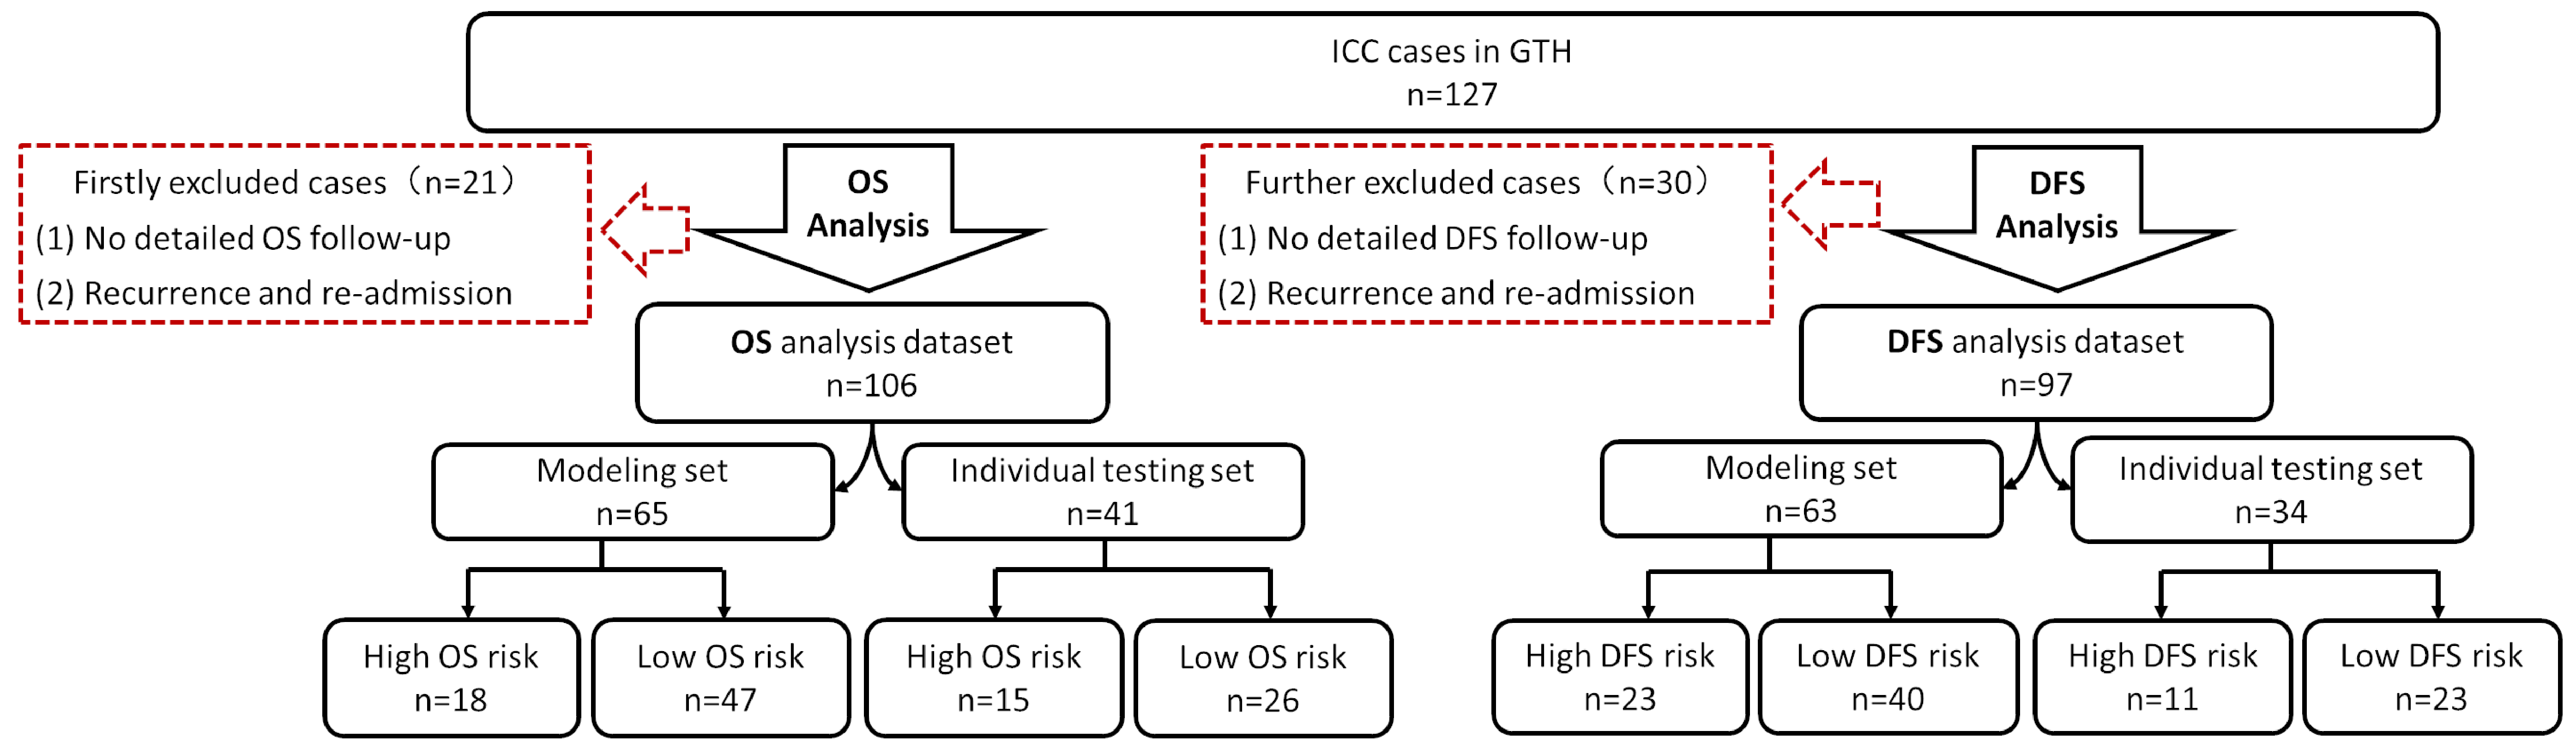
\includegraphics[scale=0.15]{FIG/fig2.eps}
\caption{Inclusion and exclusion criteria for patient selection for the modeling and test sets. Note the whole dataset with n=127 was used twice in Experiment3 on Overall survival(the left part) and Disease-Free survival analysis(the right part) respectively, see section \ref{exp3} for details. }
\label{fig2}
\end{figure}

%%%%%%%%%%%%%%%%%%%%%%%%%%%%%%%%%%%%%%%%%%%%%%%%%%%%%%%%%%% table 1
\begin{table}[]
\footnotesize
%\resizebox{0.5cm}{!}
\begin{center}
\caption{Summary of clinical and pathological features and the prediction results of cox model on overall survival where p-value of the age category was calculated by Welch’s t-test whereas the rest were calculated by Fisher exact test.}
\begin{tabular}{|l|c|c|c|}
\hline
                                               & Training set & Testing set & p-value*                \\ \hline
No. of patients                                & 65(100\%)    & 41(100\%)   & -                       \\ \hline
Age (Mean $\pm$ SD)                                & 60.63$\pm$9.67   & 59.95$\pm$10.12 & 0.2619                  \\ \hline
Sex                                            &              &             & 0.8429 \\ \cline{1-3}
\quad Male                                           & 33(50.77\%)  & 22(53.66\%) &                         \\ \cline{1-3}
\quad Female                                         & 32(49.23\%)  & 19(46.34\%) &                         \\ \hline
Tumor Number                                   &              &             & 0.4999 \\ \cline{1-3}
\quad Single                                         & 46(83.08\%)  & 32(78.5\%)  &                         \\ \cline{1-3}
\quad Multiple                                       & 19(16.92\%)  & 9(21.95\%)  &                         \\ \hline
Location                                       &              &             & 0.6934 \\ \cline{1-3}
\quad Left lobe                                      & 35(53.85\%)  & 20(48.78\%) &                         \\ \cline{1-3}
\quad Right lobe                                     & 26(40.00\%)  & 20(48.78\%) &                         \\ \hline
\quad Bilateral lobe                                 & 4(6.15\%)    & 1(2.44\%)   &                         \\ \hline
Differentiation                                &              &             & 0.7503 \\ \cline{1-3}
\quad Well                                           & 3(4.62\%)    & 2(4.87\%)   &                         \\ \cline{1-3}
\quad Moderate                                       & 48(73.85\%)  & 33(80.49\%) &                         \\ \cline{1-3}
\quad Poor                                           & 14(21.54\%)  & 6(14.63\%)  &                         \\ \hline
Tumor Max   Diameter                           &              &             & 0.1149 \\ \cline{1-3}
\quad \textgreater{}5 cm                             & 39(60.00\%)  & 21(51.22\%) &                         \\ \cline{1-3}
\quad $\leq$ 5 cm                                       & 26(40.00\%)  & 20(48.78\%) &                         \\ \hline
Peritumoral   Glisson’s Sheath Invasion (PGSI) &              &             & 0.6773 \\ \cline{1-3}
\quad Yes                                            & 24(36.92\%)  & 13(31.71\%) &                         \\ \cline{1-3}
\quad No                                             & 41(63.08\%)  & 28(68.29\%) &                         \\ \hline
micro-Vessel   Invasion (mVI)                  &              &             & 0.534  \\ \cline{1-3}
\quad Yes                                            & 23(35.38\%)  & 13(31.71\%) &                         \\ \cline{1-3}
\quad No                                             & 42(64.62\%)  & 28(68.29\%) &                         \\ \hline
TNM Stage                                      &              &             & 0.0743 \\ \cline{1-3}
\quad 1 + 2                                          & 42(64.62\%)  & 34(82.93\%) &                         \\ \cline{1-3}
\quad 3 + 4                                          & 23(35.38\%)  & 7(17.07\%)  &                         \\ \hline
IDH                                            &              &             & 0.1227 \\ \cline{1-3}
\quad Yes                                            & 10(15.38\%)  & 2(4.88\%)   &                         \\ \cline{1-3}
\quad No                                             & 55(84.61\%)  & 39(95.12\%) &                         \\ \hline
FGFR2                                          &              &             & 1.0      \\ \cline{1-3}
\quad Yes                                            & 7(10.77\%)   & 4(9.76\%)   &                         \\ \cline{1-3}
\quad No                                             & 58(89.23\%)  & 37(90.24\%) &                         \\ \hline
HBsAg (Hepatitis B surface antigen)            &              &             & 0.8222 \\ \cline{1-3}
\quad Yes                                            & 18(27.69\%)  & 10(24.39\%) &                         \\ \cline{1-3}
\quad No                                             & 47(72.31\%)  & 31(75.61\%) &                         \\ \hline
HBV infection                                  &              &             & 0.6585 \\ \cline{1-3}
\quad Yes                                            & 48(73.85\%)  & 28(68.29\%) &                         \\ \cline{1-3}
\quad No                                             & 17(26.15\%)  & 13(31.71\%) &                         \\ \hline
AFP (Alpha   fetoprotein)                      &              &             & 0.5307 \\ \cline{1-3}
\quad \textgreater{} 10 ng/ml                         & 6(9.23\%)    & 6(14.63\%)  &                         \\ \cline{1-3}
\quad $\leq$ 10 ng/ml                                      & 59(90.77\%)  & 35(85.37\%) &                         \\ \hline
CEA                                            &              &             & 1.0      \\ \cline{1-3}
\quad \textgreater{} 4 ng/ml                          & 12(18.46\%)  & 7(17.07\%)  &                         \\ \cline{1-3}
\quad $\leq$ 4 ng/ml                                       & 53(81.54\%d) & 34(82.93\%) &                         \\ \hline
CA19-9   (Carbohydrate antigen199)              &              &             & 1.0      \\ \cline{1-3}
\quad \textgreater{} 37 U/ml                          & 36(55.38\%)  & 23(56.1\%)  &                         \\ \cline{1-3}
\quad $\leq$ 37 U/ml                                       & 29(44.61\%)  & 18(43.9\%)  &                         \\ \hline
$\gamma$ GT ($\gamma$-Glutamyltransferase)                  &              &             & 0.8412 \\ \cline{1-3}
\quad \textgreater{} 50 U/ml                          & 38(58.46\%)  & 25(60.98\%) &                         \\ \cline{1-3}
\quad $\leq$ 50 U/ml                                       & 27(41.54\%)  & 16(39.2\%)  &                         \\ \hline
DBIL (Direct   bilirubin)                      &              &             & 0.0069 \\ \cline{1-3}
\quad \textgreater{} 6.8 $\mu$mol/L                       & 19(29.23\%)  & 3(7.89\%)   &                         \\ \cline{1-3}
\quad $\leq$ 6.8 $\mu$ mol/L                                    & 46(70.77\%)  & 38(92.68\%) &                         \\ \hline
TBIL (Total   bilirubin)                       &              &             & 0.003  \\ \cline{1-3}
\quad \textgreater{} 20.5 $\mu$mol /L                     & 23(35.38\%)  & 4(9.76\%)   &                         \\ \cline{1-3}
\quad $\leq$ 20.5 $\mu$ mol /L                                  & 42(64.62\%)  & 37(90.24\%) &                         \\ \hline
AST                                            &              &             & 0.0892 \\ \cline{1-3}
\quad \textgreater{} 40 U/L                           & 18(27.69\%)  & 5(7.69\%)   &                         \\ \cline{1-3}
\quad $\leq$ 40 U/L                                        & 47(72.31\%)  & 36(55.38\%) &                         \\ \hline
ALT                                            &              &             & 0.0678 \\ \cline{1-3}
\quad \textgreater{} 40 U/L                           & 20(30.77\%)  & 6(9.23\%)   &                         \\ \cline{1-3}
\quad $\leq$ 40 U/L                                        & 45(69.23\%)  & 35(53.85\%) &                         \\ \hline
AKP                                            &              &             & 0.1183 \\ \cline{1-3}
\quad \textgreater{} 185 U/L                          & 15(23.08\%)  & 4(6.15\%)   &                         \\ \cline{1-3}
\quad $\leq$ 185 U/L                                       & 50(76.92\%)  & 37(56.92\%) &                         \\ \hline
\end{tabular}
\label{Tab1}
\end{center}
\end{table}

\subsection{Computational image analysis}

\subsubsection{Tissue- and cell-levels segmentation and detection}
Tissue segmentation and lymphocyte detection are two fundamental problems of immune micro-environment analysis. The multiple tissue segmentation models in tissue-level and t-lymphocyte detection at cell-level are developed. 4 types of tissues, including liver, tumor, necrosis, and other tissues, were manually annotated by two pathologists together and finally approved by an experienced pathologist. Then tiles of $400\times400$ pixels in $100X$ magnification (0.88um/pixel) were cropped, and a total of 396 patches were obtained. The data augmentation approaches such as Flip, Rotate, and Elastic Transformation~\cite{buslaev2020albumentations} were leveraged to extend training set to 2376.

For multi-tissue segmentation at the tissue-level, standard UNet was employed for four types of tissue segmentation since UNet can balance both speed and accuracy in identifying four tissues from WSIs. For t-lymphocyte detection at cell-level, we referred to \cite{xu2015stacked} but adopted a new and more efficient solution. We trained the other UNet using an available public nuclei segmentation dataset~\cite{kumar2017dataset}. The UNet based segmentation model can obtain the boundary of each nucleus in the slide. Then morphological operations, such as the dilation and erosion, were then performed to realize the precise nucleus positioning. For each segmented nucleus, a patch of $40\times40$ pixels was obtained from the nucleus center. An AlexNet based DCNN model \cite{krizhevsky2012imagenet} was cascaded to distinguish t-lymphocyte from nuclei. The process of lymphocyte detection is much like a simplified R-CNN that replaces the selective search with nucleus segmentation and uses AlexNet to replace the SVM classifier. 

\subsubsection{Histomorphological feature extraction}
The histomorphological feature extraction pipeline is developed based on segmentation and detection results at cell- and tissue-level levels. The region of interests (ROIs) in the study was mainly focused on studying tumor-related regions. As the lymphocyte pattern is one of the most important clinical implications in the ROIs, the features at cell-level include lymphocyte distribution and their correlation with the tumor. In all, three types of features are extracted, which include the Basic Graph Features (BGFs), Clustering Graph Features (CGFs) and the Composition Features (CFs). When developing the graphs on a WSI, each lymphocyte was designated as a node in the graph. The graph's construction involves hundreds and thousands of nodes that may require more than 20GB of memory. Therefore, it is not applicable to develop a graph-based feature distribution estimation on all the detected lymphocytes in a WSI.

For tissue-level features, CFs are targeting uniting lymphocyte and tumor region. The number and the density of the lymphocyte located inside and the peri-tumoral were calculated in this feature category. The goal of these features is to do some intuitive statistical analysis.

The density map would be formed by the lymphocyte enriched regions using the sliding window in this work. The Basic Graph (BG), for example, the Voronoi graph, the Delaunay triangle, the Minimum Spanning Tree, and the Cluster Graph (CG), would be constructed map where the CG was formed though calculating the Euclidean distance between each node. In CG, each slide could aggregate several clusters in which all the nodes have the distances between each other lower than a designated thresh. Rather than using all the lymphocytes in the whole slide images, it could reduce the computation and memory consumption by designating each dense lymphocyte region as a node to build graphs. In addition to the feasibility, the density map usage ignores regions with few lymphocyte cells and concentrating on the mass distributed area, exploring the lymphocyte distribution in a more macroscopic perspective. 

\subsection{Feature selection and model construction}
Combining 3 different feature selection methods and three classifiers was used to construct the binary survival estimate model. 

In the feature selection part, mRMR\cite{peng2005feature}, t-test, and Wilcoxon Ranksum test were included. The mRMR screens the most discriminative features that could better stratify patients into the low survival group and the high by calculating the redundancy and correlation between features identified from the modeling set. From a statistical point of view, the latter two methods are taking advantage of the discrepancy of the mean value(t-test) and the rank (Wilcoxon Ranksum test) between the high-risk (HR) groups features and the low-risk (LR) group. Three top features were identified and used in the downstream studies. These features were subsequently leveraged to visualize the data points in 3-dimensional space (see Figure \ref{fig5}(b)).

%%%%%%%%%%%%%%%%%%%%%%%%%%%%%%%%%%%%%%%%%%%%%%%%%%%%%%%%%%% figure 3
\begin{figure}[h!]
\centering
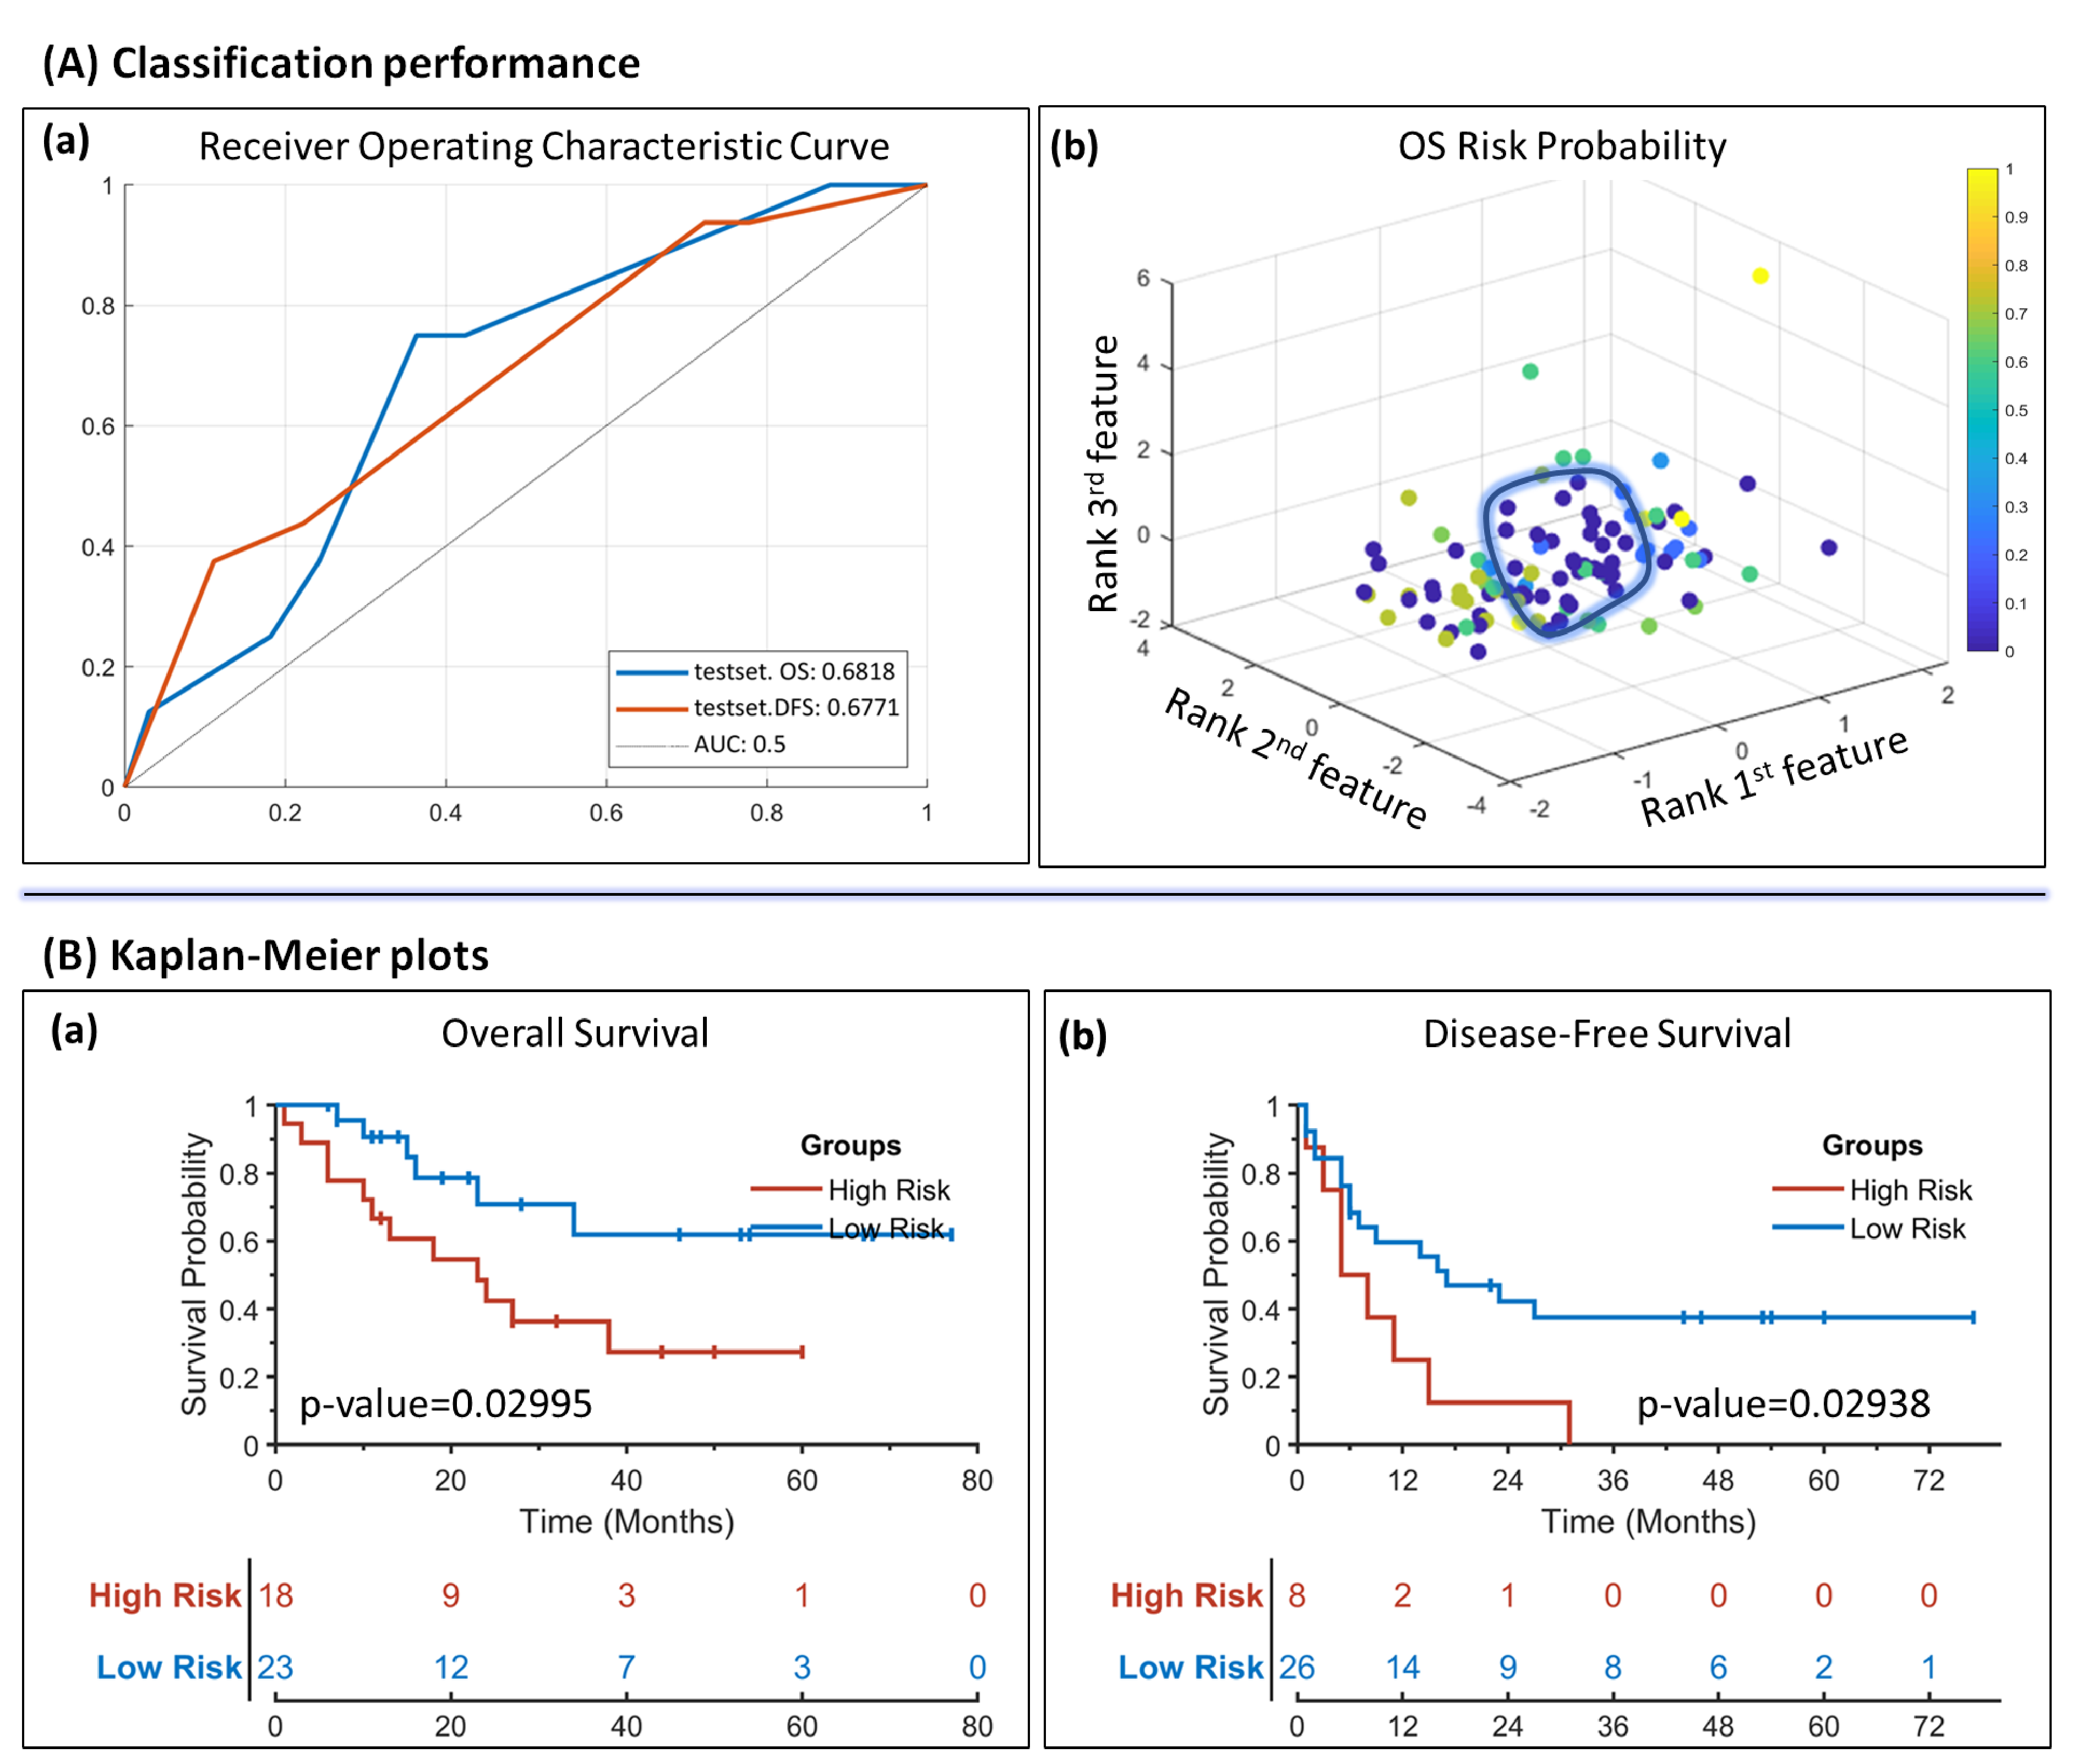
\includegraphics[scale=0.22]{FIG/fig5.eps}
\caption{Performance of our survival prediction model. (A) The classification performance plots where (a) is the Receiver Operating Characteristic (ROC) Curve where the blue line is the result of OS analysis and the red line is the DFS analysis. (b) is the 3-d plot of the selected features with the color bar represents the probability of risk, yellow means the higher probability to the end event. The higher probability(or the dark blue dots in figure) cases were most clustered within the blue polygon though the top-3 ranked features which means it will benefit classifiers to do risk stratification. (B) The Kaplan-Meier curves of the classifier where (a) is the OS plot and (b) is the DFS.}
\label{fig5}
\end{figure}

For survival estimate classifiers, linear and non-linear classifiers were implemented to better use of the selected features. In this work, a total of 3 classifiers, including Linear Discriminant Analysis (LDA), Quadratic Discriminant Analysis (QDA), and Decision Tree (DT), were picked. 

The 100 times 3-fold CV was finally adopted for evaluating the model performance and feature stability. In a total of 9 types of groups (the combination of feature selection methods and classifiers), the best-performed one was chosen for model construction by averaging the AUC of 100 iteration results. Also, in this combination, the times of the feature selected in all CV will be recorded. The most frequent one and the following two features were then be recorded to build the survival estimate model.

\subsection{Statistic survival analysis}
Once the model was trained, we further verified it on patient overall survival (OS) and the disease-free survival (DFS) information. The model will generate the probability of each patient's risk in the independent testing set, and a certain threshold will be defined in the training procedure to cut off the continuous probability into binary output (HR or LR). Additionally, features selected in OS analysis were also applied in DFS analysis to explore the feature ability and stability.

For overall survival and disease-free survival analysis, the Kaplan-Meier estimator was employed to make the line plot both HR and LR to check whether our model could give the objective output. The log-rank test will be applied in a quantitative method to determine the significance between binary output and patient survival. Then, to compare the traditional survival indicators such as the TNM staging and the micro-vessel invasion status, multivariate Cox proportional hazard models were also used to get the hazard rate between different survival predictors. 

All the statistic tools used in this work were two-tailed, with the significance level under 0.05. All the p values were calculated using packages including ‘survival’ (https://cran.r-project.org/web/packages/survival/index.html) and ‘survminer’ (https://cran.r-project.org/web/packages/survminer/index.html) of R with version 3.6.3. All the KM plot figure were plotted using the library ‘MatSurv’(https://github.com/aebergl/MatSurv)

\section{Experimental results and discussion}\label{result}
Figure \ref{fig3} shows the qualitative results of tissue segmentation (Figure \ref{fig3}(b,c)) and t-lymphocyte detection (Figure \ref{fig3}(d,e)) results in cell-and tissue levels on a whole slide image (Figure \ref{fig3}(a)), respectively. The Dice coefficient and the F1-score (follow the method in \cite{sirinukunwattana2016locality}) was applied for quantitatively evaluating the tissue segmentation and the t-lymphocyte detection, respectively. Table \ref{Tab2} shows results in terms of the above metrics. For multiple tissue segmentation, the pixel accuracy is around 90\%, except for the others with 87.2\%, and the overall dice coefficient is 0.8603. For t-lymphocyte detection, the model got the F1-score of 0.8295 and a higher precision value of 0.8871 than the recall of 0.7791, which means our detection model can reduce false positive (also called misdetection) results. 

%%%%%%%%%%%%%%%%%%%%%%%%%%%%%%%%%%%%%%%%%%%%%%%%%%%%%%%%%%% figure 4
\begin{figure}[h!]
\centering
\includegraphics[scale=0.21]{FIG/fig3.eps}
\caption{Qualitative results of tissue segmentation (b,c) and t-lymphocyte detection on a whole slide image of ICC (a). (b) is the full view of the segmentation and detection result respectively wherein (b), the red region is the segmented liver, green in is the tumor, blue is necrosis and black is the other components in slides and in (d), white dots represent the detected t-lymphocyte; (c, e) is the zoomed window with mapping the segmentation(c) and detection(e) results over the original H\&E stained image patch.}
\label{fig3}
\end{figure}

%%%%%%%%%%%%%%%%%%%%%%%%%%%%%%%%%%%%%%%%%%%%%%%%%%%%%%%%%%% table 2
\begin{table}[htbp]
  \centering
  \caption{Detailed evaluation metrics of the segmentation and detection.}
    \begin{tabular}{|c|p{5.535em}c|c|}
    \toprule
    \multicolumn{1}{|p{5.25em}|}{\textbf{Pipeline}} & \multicolumn{2}{p{11.5em}|}{\textbf{Metrics}} & \multicolumn{1}{p{5.5em}|}{\textbf{Performance}} \\
    \midrule
    \multicolumn{1}{|c|}{\multirow{5}[10]{*}{Multi-tissue segmentation}} & \multicolumn{2}{p{11.5em}|}{Overall DICE coefficient} & 0.8603 \\
\cmidrule{2-4}          & \multicolumn{1}{c|}{\multirow{4}[8]{*}{Pixel Accuracy}} & \multicolumn{1}{p{6.20em}|}{Liver region} & 97.43\% \\
\cmidrule{3-4}          & \multicolumn{1}{c|}{} & \multicolumn{1}{p{6.20em}|}{Tumor region} & 90.39\% \\
\cmidrule{3-4}          & \multicolumn{1}{c|}{} & \multicolumn{1}{p{6.20em}|}{Necrosis region} & 98.12\% \\
\cmidrule{3-4}          & \multicolumn{1}{c|}{} & \multicolumn{1}{p{6.20em}|}{Others region} & 87.20\% \\
    \midrule
    \multicolumn{1}{|c|}{\multirow{3}[6]{*}{t-lymphocyte detection}} & \multicolumn{2}{p{11.5em}|}{Precision} & 0.8871 \\
\cmidrule{2-4}          & \multicolumn{2}{p{11.5em}|}{Recall} & 0.7791 \\
\cmidrule{2-4}          & \multicolumn{2}{p{11.5em}|}{F1-score} & 0.8295 \\
    \bottomrule
    \end{tabular}%
  \label{Tab2}%
\end{table}%
 
\subsection{Experiment 1: Identifying TIL related features}
After applying 100 times 3-fold cross-validation (CV) on the modeling set, the top 3 features selected by mRMR were shown in Table \ref{Tab3}. 

%%%%%%%%%%%%%%%%%%%%%%%%%%%%%%%%%%%%%%%%%%%%%%%%%%%%%%%%%%% table 3
\begin{table}[htbp]
  \centering
  \caption{The top 3 selected features identified from modeling set for statistic survival analysis.}
    \begin{tabular}{|c|c|c|c|}
    \toprule
    \multicolumn{1}{|p{8.57em}|}{\textbf{Feature category}} & \multicolumn{1}{p{4.001em}|}{\textbf{Feature ranking}} & \multicolumn{1}{p{8.0em}|}{\textbf{Feature name}} & \multicolumn{1}{p{8.0em}|}{\textbf{Simple description}} \\
    \midrule
    \multicolumn{1}{|c|}{\multirow{2}[2]{*}{\makecell[c]{Cluster graph features\\(CGFs)}}} & \multicolumn{1}{c|}{\multirow{2}[2]{*}{1st}} & \multicolumn{1}{c|}{\multirow{2}[2]{*}{Edge statistics}} & \multicolumn{1}{l|}{\multirow{2}[2]{*}{\makecell[l]{The standard deviation of the length of \\edges}}} \\
          &       &       &  \\
    \midrule
    \multicolumn{1}{|c|}{\multirow{2}[2]{*}{\makecell[c]{Basic graph features\\(BGFs)}}} & \multicolumn{1}{c|}{\multirow{2}[2]{*}{2nd}} & \multicolumn{1}{c|}{\multirow{2}[2]{*}{Around distribution}} & \multicolumn{1}{l|}{\multirow{2}[2]{*}{\makecell[l]{Disorder of the distance of the nearest \\ neighbors in a circle with a 10-pixel radius}}} \\
          &       &       &  \\
    \midrule
    \multicolumn{1}{|c|}{\multirow{2}[2]{*}{\makecell[c]{Composition features\\(CFs)}}} & \multicolumn{1}{c|}{\multirow{2}[2]{*}{3rd}} & \multicolumn{1}{c|}{\multirow{2}[2]{*}{Density of lymphocyte}} & \multicolumn{1}{l|}{\multirow{2}[2]{*}{\makecell[l]{The density of lymphocyte within \\the peri-tumor region (18-pixels outside)}}} \\
          &       &       &  \\
    \bottomrule
    \end{tabular}%
  \label{Tab3}%
\end{table}%

The three selected features fall into three different feature categories. The first feature is edge statistics, which calculates the length of edges in the CG and use the standard deviation to evaluate the nodes' disorder in clusters. The higher this feature, the higher heterogeneity of clusters. Then, the second feature is around distribution features belonging to the BGFs. It described the distribution of the lymphocyte dense regions at a micro-level. Besides the distribution, composition analysis was also included in our feature set. A vivid illustration figure was shown in Figure \ref{fig4}(a). The last feature selected is the signature of the lymphocyte density within the peripheral of the tumor glands, where the outer boundary was 18 pixels (15.6um) away from the boundary of the tumor glands. The corresponding KM plots are shown in Figure \ref{fig4}(b) with the log-rank test p-value of 0.01385. All these features selected were then combined with DT to build the survival estimation model.

%%%%%%%%%%%%%%%%%%%%%%%%%%%%%%%%%%%%%%%%%%%%%%%%%%%%%%%%%%% figure 5
\begin{figure}[h!]
\centering
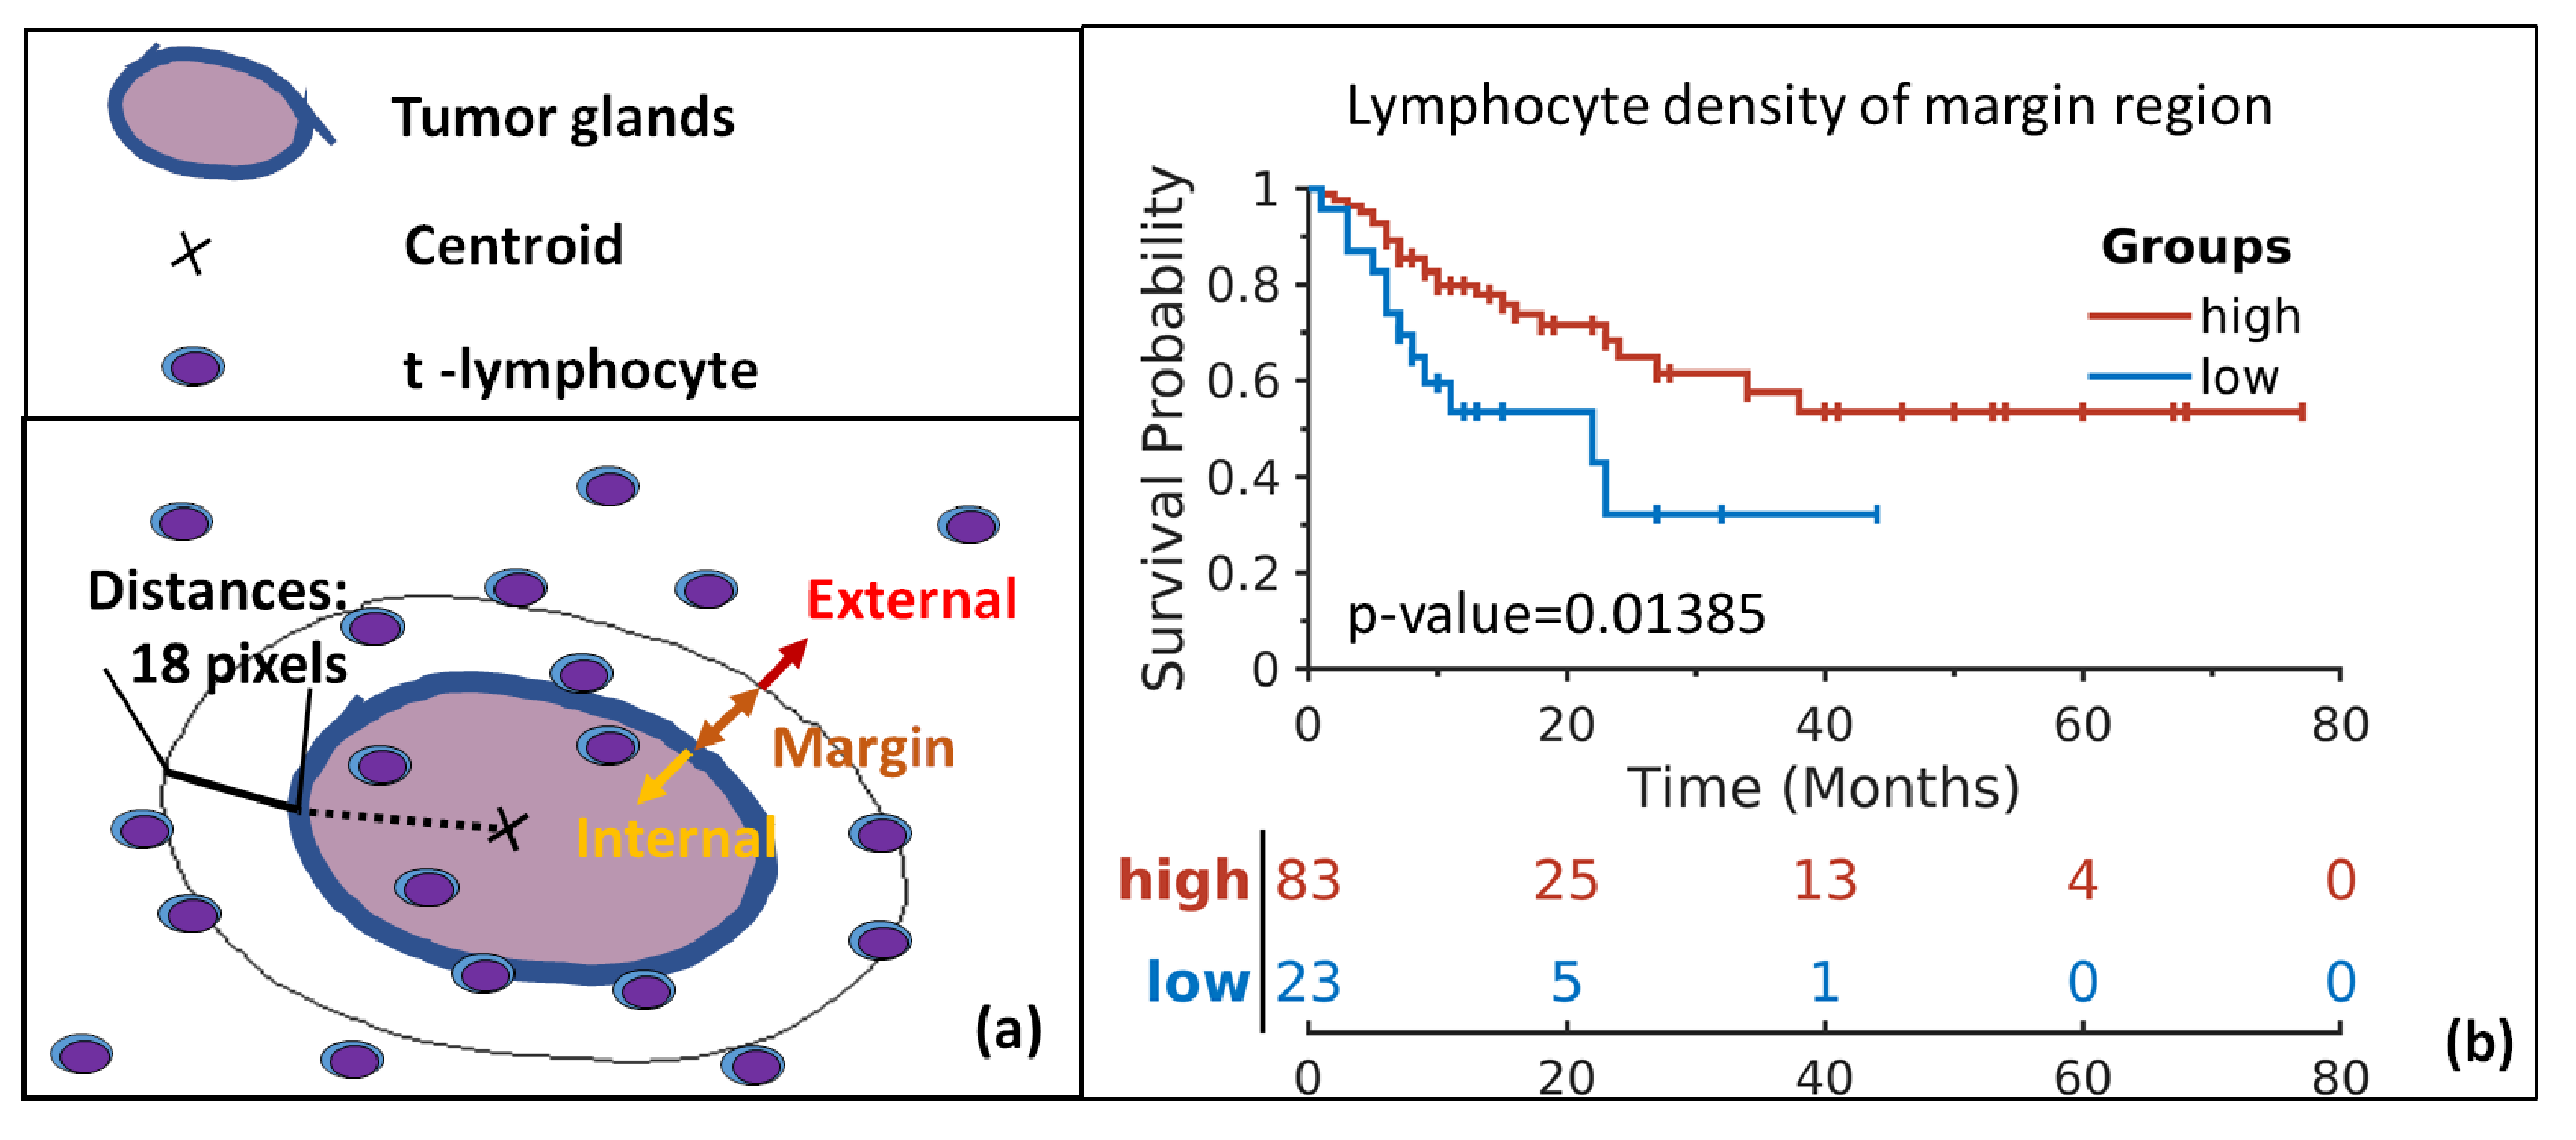
\includegraphics[scale=0.24]{FIG/fig4.eps}
\caption{Feature explanation on (a) illustrating the definition of the around distribution feature. (b) showing the KM plot of the second selected feature using the method of p-value minimization.}
\label{fig4}
\end{figure}

\subsection{Experiment 2: Assessing the prognostic significance of features}
\label{exp3}
A total of 106 patients were included in our experiment. The average age was 60.63$\pm$9.67 and 59.95$\pm$10.12 in the modeling set and independent testing set. Some clinical, pathological and serological signatures that are likely correlated with patient survival were listed in Table 1. The p-value was calculated by the two-tailed Fisher exact test (discrete variables) and Welch’s t-test (continuous variables without homoscedasticity). 

Figure \ref{fig5} shows the performance of our survival prediction model in two parts where the upper half illustrates the Receiver Operating Characteristic (ROC) Curve (Figure \ref{fig5}A(a)) and the scatter plot of all the data points in the testing set with the predicted survival risk color bar(Figure \ref{fig5}A(b)). In the ROC curve, the AUC of the overall OS analysis on the independent testing set is 0.6818, and the AUC of DFS analysis is 0.6771. From the results, the OS and DFS estimation model trained with the same features have a similar performance, which is an indicator that these features have robustness. For the right part of Figure \red{fig5}A, each point's location in this figure is defined by three ranked feature values. The colors are determined by our survival prediction model's output, where yellow means HR's probability, whereas blue represents the LR. The second half is the Kaplan-Meier curves of the survival prediction model on OS (Figure \ref{fig5}B(a)) and DFS (Figure \ref{fig5}B(b)) with the log-rank test p-value of 0.02995 and 0.02938, respectively.


Although the univariant analysis could verify the prediction model's effectiveness, the independent predict performance compared with traditional survival-related signatures is still puzzled. All the other univariant analysis result which is not significant in 95\% confidence interval were shown in  materials 2. Table \ref{Tab4} shows that the OS model is an independent survival predictor compared with the PGSI, TNM staging and $\gamma$GT with multivariant Cox hazard model p-value of 0.0475 and the hazard ratio of 2.9 (95\% confidence interval: 1.01–8.32). However, in DFS analysis, the 3 features-supported models trained was instead of an independent signature, which means that the model trained on DFS was a recurrence-related indicator. The traditional TNM staging is still a powerful recurrence signature.

%%%%%%%%%%%%%%%%%%%%%%%%%%%%%%%%%%%%%%%%%%%%%%%%%%%%%%%%%%% table 4
\begin{table}[htbp]
  \centering
  \caption{Multivariate Cox proportional hazard model analysis results.}
    \begin{tabular}{llllll}
    \toprule
    \multicolumn{1}{|c|}{\multirow{2}[4]{*}{\textbf{Types}}} & \multicolumn{1}{c|}{\multirow{2}[4]{*}{\textbf{Signatures}}} & \multicolumn{2}{c|}{\textbf{Cox Univariant*}} & \multicolumn{2}{c|}{\textbf{Cox Multivariant}} \\
\cmidrule{3-6}    \multicolumn{1}{|c|}{} & \multicolumn{1}{c|}{} & \multicolumn{1}{c|}{p-value} & \multicolumn{1}{p{8.00em}|}{HR (95\% CI)} & \multicolumn{1}{c|}{p-value} & \multicolumn{1}{p{8.00em}|}{HR (95\% CI)} \\
    \midrule
    \multicolumn{1}{|c|}{\multirow{4}[8]{*}{\makecell[c]{OS\\(N=106)}}} & \multicolumn{1}{l|}{PGSI} & \multicolumn{1}{c|}{0.022} & \multicolumn{1}{p{8.00em}|}{3.07 (1.18 - 7.99)} & \multicolumn{1}{c|}{0.7109} & \multicolumn{1}{p{8.00em}|}{2.23 (0.61 - 8.13)} \\
\cmidrule{2-6}    \multicolumn{1}{|c|}{} & \multicolumn{1}{l|}{TNM (1+2 vs. 3+4)} & \multicolumn{1}{c|}{0.0336} & \multicolumn{1}{p{8.00em}|}{3.21 (1.09 - 9.42)} & \multicolumn{1}{c|}{0.224} & \multicolumn{1}{p{8.00em}|}{1.29 (0.33 - 5.034)} \\
\cmidrule{2-6}    \multicolumn{1}{|c|}{} & \multicolumn{1}{l|}{$\gamma$GT} & \multicolumn{1}{c|}{0.021} & \multicolumn{1}{p{8.00em}|}{3.78 (1.22 - 11.69)} & \multicolumn{1}{c|}{0.1399} & \multicolumn{1}{p{8.00em}|}{2.53 (0.74 - 8.67)} \\
\cmidrule{2-6}    \multicolumn{1}{|c|}{} & \multicolumn{1}{l|}{\textbf{Image-based Model}} & \multicolumn{1}{c|}{\textbf{0.0314}} & \multicolumn{1}{p{8.00em}|}{\textbf{2.83 (1.06 - 7.55)}} & \multicolumn{1}{c|}{\textbf{0.0475}} & \multicolumn{1}{p{8.00em}|}{\textbf{2.90 (1.01 - 8.32)}} \\
    \midrule
    \multicolumn{1}{|c|}{\multirow{4}[8]{*}{\makecell[c]{DFS\\(N=97)}}} & \multicolumn{1}{l|}{\textbf{TNM (1+2 vs. 3+4)}} & \multicolumn{1}{c|}{\textbf{0.044}} & \multicolumn{1}{p{8.00em}|}{\textbf{3.33 (1.03 - 10.72)}} & \multicolumn{1}{c|}{\textbf{0.0152}} & \multicolumn{1}{p{8.00em}|}{\textbf{4.78 (1.35 - 6.89)}} \\
\cmidrule{2-6}    \multicolumn{1}{|c|}{} & \multicolumn{1}{l|}{DB} & \multicolumn{1}{c|}{0.0439} & \multicolumn{1}{p{8.00em}|}{5.08 (1.05 - 24.67)} & \multicolumn{1}{c|}{0.0698} & \multicolumn{1}{p{8.00em}|}{4.68 (0.88 – 24.86)} \\
\cmidrule{2-6}    \multicolumn{1}{|c|}{} & \multicolumn{1}{l|}{$\gamma$GT} & \multicolumn{1}{c|}{0.0463} & \multicolumn{1}{p{8.00em}|}{2.49 (1.02 - 6.1)} & \multicolumn{1}{c|}{0.0485} & \multicolumn{1}{p{8.00em}|}{2.59 (1.01 - 6.67)} \\
\cmidrule{2-6}    \multicolumn{1}{|c|}{} & \multicolumn{1}{l|}{Image-based Model} & \multicolumn{1}{c|}{0.0354} & \multicolumn{1}{p{8.00em}|}{2.56 (1.07 - 6.128)} & \multicolumn{1}{c|}{0.1569} & \multicolumn{1}{p{8.00em}|}{1.89 (0.78 – 4.59)} \\
    \midrule
    \multicolumn{6}{l}{\multirow{2}[1]{*}{\makecell[l]{*All the other univariant analysis result which is not significant in 95\% confidence interval were shown \\in supplementary materials 1.}}} \\
    \multicolumn{6}{l}{} \\
    \end{tabular}%
  \label{Tab4}%
\end{table}%

Furthermore, to better understand the features identified, figure \ref{fig6} visualizes the CGF in the HR and LR. For HR patients in the left red rectangle, the dense lymphocyte region is surrounded by the whole tumor. Although some nodes spread inside the central part of the tumor (the black dots in the figure, which is the isolated node that the distance to the nearest node is larger than the distance threshold in the cluster), these points may not be enough to form a strong anti-tumor ‘army’ if considering quantity. The dense points are relatively uniformly distributed for LR patient in the green rectangle, compared to the left rectangle slide. In detail, Figure \ref{fig6}(c, d) demonstrate the histogram plot of the edge length. The short edges and the median edges are more frequently appears in the LR slide, whereas only short edges in the HR slide show that the nodes in the HR slides will have a high probability of getting together (not necessarily around the tumor boundary like Figure \ref{fig6}(a)) rather than the large scale mixed distribution.

%%%%%%%%%%%%%%%%%%%%%%%%%%%%%%%%%%%%%%%%%%%%%%%%%%%%%%%%%%% figure 6
\begin{figure}[h!]
\centering
\includegraphics[scale=0.22]{FIG/fig6.eps}
\caption{Feature visualization of the CGFs. (a, b) is the original whole slide image covered with the cluster graphs where each convex polygon is one cluster. The left half which in the red rectangle is a patient with High-risk and the right part in the green rectangle is Low-risk. The colored dots represent the dense lymphocyte regions and those black are isolated which do not make up any clusters. (c-d) is the edge statistic demonstration of the second selected feature using the 20 bins histogram plot.}
\label{fig6}
\end{figure}

Intrahepatic cholangiocarcinoma is a highly heterogeneous and lethal malignant tumor. Histological evaluation and TNM staging based on surgically resected specimens are currently the main ways to predict the prognosis of patients\cite{bird2018meta}. However, ICC pathologically has significant heterogeneity in patterns of tumoral cells, fibroblasts and immune cells\cite{dong2018spatial}. Traditional pathology only finds limited features for tumor morphology through human vision, such as glandular differentiation and mitotic activity, and they cannot be characterized quantitatively\cite{bera2019artificial,madabhushi2016image}. Understanding the interrelationship between ICC tumors and host immune status is becoming increasingly important to understand malignant tumors. A large amount of recent evidence indicates that the tumor immune microenvironment strongly determines the prognosis of tumors\cite{2019Superpixel}. For example, tumor-infiltrating lymphocyte (TIL) is an essential indicator for evaluating the tumor immune microenvironment, and a large number of studies show that it has a crucial significance in the evaluation of tumor prognosis\cite{pages2018international}.
	
In this study, we aimed at finding the independent survival predictor of ICC patients from the digitized H\&E stained whole slide images using the machine learning-based classifier. In the pipeline of building the survival risk classifier, deep learning-based multiple tissue segmentation and t-lymphocyte detection were first employed. Then lymphocyte and tumor-related sub-visual features, including the BGFs, CGFs, and CFs, were designed and extracted in the whole slide images.

Though there exist many previous computer-aid image analysis method that quantifies the relationship between the survival and the image patterns in many other cancers, these methods still did not provide a solution for the pathologist to have a vivid impression to understand the results of their model from the perspective of the whole slide images. Kather et al. \cite{kather2018topography} showed the usage of immunohistochemistry to quantify the tumor microenvironment and defined patterns of the immune type which could stratify patients' survival risk. It provides a research framework to investigate immunotherapy responsiveness in clinical trials but does not translate these patterns into understandable visual concepts. For example, the concept of nucleus enlargement is the symptom of nucleus heteromorphism. Secondly, TILs is a highly spotted tumor research field, and it is a straightforward idea to do some statistical analysis on the composition or the lymphocytes' location about the tumor. Zormpas-Petridis et al. \cite{zormpas2019superpixel} evaluated the statistics of cell composition in whole slide images, including the ratio of stromal cells to all cells and the ratio of lymphocytes located internally of the tumor to all lymphocytes. We assessed its prognosis value in TCGA cohorts of patients with melanoma.

Further, Yuan et al. \cite{yuan2015modelling} demonstrated the idea that the mapping of the spatial distribution of the different kinds of lymphocytes in tumor sections is a valuable tool to characterize patients' survival with triple-negative breast cancer. Other studies were trying to use some mathematical methods to characterize the lymphocyte distribution. However, much of these works were applied to tissue microarray. For example, Corredor et al. \cite{2013Spatial} modeled the density and spatial architecture of TILs with the 'spaTIL' feature set and validated them in recurrence of early-stage in non-small cell lung cancer. Saltz et al. \cite{saltz2018spatial}did the whole slide-level clustering distribution analysis of TILs, but we further take the tumor glands into account rather than the whole tumor region in the composition analysis.

Limitations are also concluded. Firstly, the total number of cases in training and testing cohorts is slightly insufficient in survival analysis, which contributes to some prognostic significant pathological indicators in ICC, such as the status of mVI, CA19-9, were not counted. Further studies will be continued for validating the effectiveness of these features in multi-center together with robust statistical methods for investigating more hidden patterns of this kind of malignant tumor. Secondly, whole slide-level registration (pixel-level alignment of serial sections) will be employed to solve the difficulty of morphology difference in serial sections, which will be available to consider the different subsets of lymphocytes to analyze TILs economically and efficiently. 

A computer-assisted survival estimator based on a machine learning classifier can predict patient survival in ICC. More importantly, these features that quantitatively describe the distribution of lymphocytes are mostly explainable and could be translated into pathological descriptions. These results laid the foundation for further research to expand the ability of the computer aid prognostic predictor. 

\section{Conclusions}\label{conclusion}
This work presents a quantitative solution to assess the lymphatic infiltration status in the tumor environment. Through this method, we find a series of features that can predict the overall survival of Intrahepatic cholangiocarcinoma(ICC) patients and suggest the prognosis of disease-free survival. The quantitative evaluation results demonstrate that our method can help pathologists make decisions on overall survival compared to traditional clinical signatures. Also, in the feature visualization part, results show significant visual variations between high/low-risk slides. In summary, we present a new method to find visual patterns or features that create a possibility to explore the reasons between tumor infiltrating lymphocytes and the ICC tumor and better assesses prognosis.

\section*{Ethical approval}
In all participants, the informed consent to be included in the research was obtained and the Ethical Committee of the Hospital approved the protocol.

\section*{Declaration of Competing Interest}
The authors declare no conflict of interest.

\section*{Acknowledgements}
Research reported in this publication was partially supported by National Natural Science Foundation of China (Nos. U1809205, 61771249, 91959207, 81871352, 81802394, 61672334, 61502290, 61401263); Natural Science Foundation of Jiangsu Province of China (No. BK20181411); Fundamental Research Funds for the Central Universities (201903096, GK201901010). The 14th Six Talent Peaks Project in Jiangsu Province (WSW-073), and the 13th Five-year Nanjing Health Youth Training Project, (QRX17055). Dr. Madabhushi was partially supported by the National Cancer Institute of the National Institutes of Health under award numbers: 1U24CA199374-01, R01CA202752-01A1, R01CA208236-01A1, R01 CA216579-01A1, R01 CA220581-01A1, 1U01 CA239055-01. National Center for Research Resources under award number1-C06-RR12463-01VA Merit Review Award IBX004121A from the United States Department of Veterans Affairs Biomedical Laboratory Research and Development Service, The DoD Breast Cancer Research Program Breakthrough Level 1 Award W81XWH-19-1-0668, The DOD Prostate Cancer Idea Development Award (W81XWH-15-1-0558), The DOD Lung Cancer Investigator-Initiated Translational Research Award (W81XWH-18-1-0440), The DOD Peer Reviewed Cancer Research Program (W81XWH-16-1-0329), The Ohio Third Frontier Technology Validation Fund, The Wallace H. Coulter Foundation Program in the Department of Biomedical Engineering and The Clinical and Translational Science Award Program (CTSA) at Case Western Reserve University. The content is solely the responsibility of the authors and does not necessarily represent the official views of the National Institutes of Health, the U.S. Department of Veterans Affairs, the Department of Defense, or the United States Government. Dr. Lu is partially supported by the The DoD Breast Cancer Research Program Breakthrough Level 1 Award W81XWH-19-1-0668.

\section*{Author contributions statement}
Conception and Design: Jun Xu, Jun Chen, Xiangshan Fan, Jiawei Xie, Anant Madabhushi. Development of methodology: Jun Xu, Jun Chen, Jiawei Xie.
Acquisition of data: Jun Chen, Xiangshan Fan, Xiaohong Pu, Yudong Qiu, Jian He, Jiong Shi, Yuemei Xu.
Analysis and data interpretation: Jiawei Xie, Xiaohong Pu, Yudong Qiu, Jian He, Cheng Lu, Wei Gao, Haoda Lu, Anant Madabhushi. Writing, review, and/or revision of the manuscript: All authors. Jun Xu and Jun Chen are the corresponding authors, and confirm that all authors have seen and approved of the final text. All authors reviewed the manuscript. 

\printendnotes

% Submissions are not required to reflect the precise reference formatting of the journal (use of italics, bold etc.), however it is important that all key elements of each reference are included.
\bibliography{ICC}

%\begin{biography}[example-image-1x1]{A.~One}
%Please check with the journal's author guidelines whether %author biographies are required. They are usually only included %for review-type articles, and typically require photos and %brief biographies (up to 75 words) for each author.
%\bigskip
%\bigskip
%\end{biography}

%\graphicalabstract{example-image-1x1}{Please check the journal's author guildines for whether a graphical abstract, key points, new findings, or other items are required for display in the Table of Contents.}

\end{document}